\chapter{Parallel Monte Carlo Synthetic Acceleration}
\label{ch:parallel_methods}
For MCSA to be viable at the production scale, scalable parallel
implementations of the algorithm are required. Reviewing the
literature, MCSA has yet to be parallelized and the Neumann-Ulam Monte
Carlo method on which it is built has only been parallelized through
history-level parallelism with full domain replication. In order to
solve large linear systems with MCSA, a domain-decomposed parallel
strategy is required. In the formulation of a parallel MCSA algorithm,
we recognize that the algorithm occurs in two stages, an outer
iteration performing fixed point iteration and applying the
correction, and an inner Monte Carlo solver that is generating the
correction via the adjoint or forward methods. The parallel aspects of
both these components must be considered. Therefore, we will develop
and implement parallel algorithms for the Neumann-Ulam and MCSA
methods leveraging both the knowledge gained from the general parallel
implementations of Krylov methods reviewed in
Appendix~\ref{ch:linear_problem} and modern parallel strategies for
domain decomposed Monte Carlo as developed by the reactor physics
community.

In this chapter we briefly review particle transport methods for
domain decomposed Monte Carlo. Considering a domain decomposed
Neumann-Ulam method, we derive an analytic framework based on
algebraic quantities from which to estimate its performance when
applied to linear systems. We then devise a parallel algorithm for the
Neumann-Ulam method based on the multiple-set overlapping-domain
decomposition algorithm and a parallel algorithm for the MCSA that
leverages the parallel Monte Carlo algorithm and general parallel
matrix-vector operations. In identical fashion to the serial
computations presented in Chapter~\ref{ch:spn_equations}, we use
parallel solutions for the $SP_N$ equations for the fuel assembly
criticality problem to verify the correctness of the parallel
algorithm and implementation by comparing the numerical results
against production Krylov methods. Using the verified implementation
of the algorithm, we perform parallel scaling studings to test its
performance on both a small computing cluster and a leadership class
machine and compare this performance to the production Krylov methods.

%%---------------------------------------------------------------------------%%
\section{Domain Decomposed Monte Carlo}
\label{sec:msod}
As observed in the discussion on parallel Krylov methods in
Appendix~\ref{ch:linear_problem}, large-scale problems will surely
have their data partitioned such that each parallel process owns a
subset of the equations in the linear system. Given this convention,
the Neumann-Ulam Monte Carlo algorithm must perform random walks over
a domain that is decomposed and must remain decomposed due to memory
limitations. This naturally leads us to seek parallel Monte Carlo
algorithms that handle domain decomposition.

\begin{figure}[t!]
  \begin{center}
    \scalebox{1.5}{
      \input{chapters/parallel_mc/ddmc_example.pdftex_t} }
  \end{center}
  \caption{\textbf{Domain decomposed Monte Carlo transport example
      illustrating how domain decomposition requires parallel
      communication of particles.}}
  \label{fig:ddmc_example}
\end{figure}

\begin{figure}[t!]
  \begin{center}
    \scalebox{1.5}{
      \input{chapters/parallel_mc/ddnu_example.pdftex_t} }
  \end{center}
  \caption{\textbf{Domain decomposed Neumann-Ulam example illustrating
      how domain decomposition requires parallel communication of
      histories.} \textit{Each mesh point corresponds to an equation
      in the linear system and the coupling among equations is
      described by the discretization of the problem.}}
  \label{fig:ddnu_example}
\end{figure}

\clearpage

%%---------------------------------------------------------------------------%%
\section{Analytic Performance Framework for Domain-Decomposed Monte Carlo}
\label{sec:analytic_framework}
To date, parallel Neumann-Ulam methods have been limited to full
domain replication with parallelism exploited through individual
histories \citep{alexandrov_efficient_1998} and in this chapter we
will exploit particle transport algorithms to alleviate this. To
accomplish this, we recognize from the literature that stochastic
histories must be transported from domain to domain as the simulation
progresses and they transition to states that are not in the local
domain. Because we have chosen a domain decomposition strategy in a
parallel environment, this means that communication of these histories
must occur between compute nodes owning neighboring pieces of the
global domain. We wish to characterize this communication not only
because communication is in general expensive, but also because these
nearest-neighbor communication sequences, specifically, have poor
algorithmic strong scaling \citep{gropp_high-performance_2001} in much
the same way as a matrix-vector multiply operation. Therefore, we
desire a framework to provide a simple, analytic theory based on the
properties of the linear system that will allow for estimates of the
domain decomposed behavior of the Neumann-Ulam method in terms of the
amount of information that must be communicated.

When solving problems where the linear operator is symmetric, a host
of analytic theories exist based on the eigenvalue spectrum of the
operator that characterize their behavior in the context of
deterministic linear solvers. Using past work, these theories are
adapted to the domain decomposed Neumann-Ulam method using the
one-speed, two-dimensional neutron diffusion equation and spatial
discretization presented in
Appendix~\ref{chap:diffusion_problem}. Using the linear system
generated by the discretization of the model problem, we use a
spectral analysis to generate analytic relations for the eigenvalues
of the operator based on system parameters. Using the eigenvalue
spectra, we then build relationships to characterize the transport of
stochastic histories in a decomposed domain and the fraction of
histories that leak from a domain and will therefore have to be
communicated. Finally, we compare these analytic results to numerical
experiments conducted with the model problem.

\subsection{Spectral Analysis}
\label{subsec:spectral_analysis}
The convergence of the Neumann series in
Eq~(\ref{eq:adjoint_neumann_series}) approximated by the Monte Carlo
solver is dependent on the eigenvalues of the iteration matrix. We
will compute these eigenvalues by assuming eigenfunctions of the form
\citep{leveque_finite_2007}:
\begin{equation}
  \Phi_{p,q}(x,y) = e^{2 \pi \imath p x} e^{2 \pi \imath q y}\:,
  \label{eq:eigenfunction_form}
\end{equation}
where different combinations of $p$ and $q$ represent the different
eigenmodes of the solution. As these are valid forms of the solution,
then the action of the linear operator on these eigenfunctions should
give the eigenvalues of the matrix as they exist on the unit circle in
the complex plane.

For the model problem, we first compute the eigenvalues for the
diffusion operator $\ve{D}$ by applying the operator to the
eigenfunctions and noting that $x=ih$ and $y=jh$:
\begin{multline}
  \ve{D}\Phi_{p,q}(x,y) = \lambda_{p,q}(\ve{D})
  =\\ -\frac{D}{6h^2}\Big[4 e^{-2 \pi \imath p h} + 4 e^{2 \pi \imath
      p h} + 4 e^{-2 \pi \imath q h} + 4 e^{2 \pi \imath q h} + e^{-2
      \pi \imath p h} e^{-2 \pi \imath q h} \\ + e^{-2 \pi \imath p h}
    e^{2 \pi \imath q h} + e^{2 \pi \imath p h} e^{-2 \pi \imath q h}
    + e^{2 \pi \imath p h} e^{2 \pi \imath q h} - 20\Big] + \Sigma_a
  \:.
  \label{eq:deriv_diff_1}
\end{multline}
Using Euler's formula, we can collapse the exponentials to
trigonometric functions:
\begin{equation}
  \lambda_{p,q}(\ve{D}) = -\frac{D}{6h^2}[ 8 \cos(\pi p h) + 8
    \cos(\pi q h) + 4 \cos(\pi p h) \cos(\pi q h) - 20] + \Sigma_a\:.
  \label{eq:deriv_diff_2}
\end{equation}

As Eq~(\ref{eq:diffusion_eq}) is diagonally dominant, point Jacobi
preconditioning as outlined in
\S~\ref{subsec:stochastic_preconditioning} is sufficient to reduce the
spectral radius of the iteration matrix below unity and therefore
ensure convergence of the Neumann series. Applying this
preconditioner, we are then solving the following diffusion system:
\begin{equation}
  \ve{M}^{-1} \ve{D} \boldsymbol{\phi} = \ve{M}^{-1} \ve{s}\:.
  \label{eq:precond_diffsion}
\end{equation}
The operator $\ve{M}^{-1} \ve{D}$ is merely the original diffusion
operator with each row scaled by the diagonal component. As we have
defined a homogeneous domain, the scaling factor, $\alpha$, is the
same for all rows in the operator and defined as the $\phi_{i,j}$
coefficient from Eq~(\ref{eq:fd_system}):
\begin{equation}
  \alpha = \Bigg[\frac{10 D}{3 h^2} + \Sigma_a\Bigg]^{-1}\:.
  \label{eq:jacobi_scaling}
\end{equation}
Using this coefficient, we then have the following spectrum of
preconditioned eigenvalues:
\begin{equation}
  \lambda_{p,q}(\ve{M}^{-1} \ve{D}) = \alpha \lambda_{p,q}(\ve{D})\:.
  \label{eq:preconditioned_eigenvalues}
\end{equation}

The spectral radius of the iteration matrix is obtained by seeking its
largest eigenvalue. As with the diffusion operator, we can use the
same analysis techniques to find the eigenvalues for the iteration
matrix. We use a few simplifications by noting that if the Jacobi
preconditioned iteration matrix is $\ve{H} = \ve{I} -
\ve{M}^{-1}\ve{D}$, the we except all terms on the diagonal of the
iteration matrix to be zero such that we have the following stencil:
\begin{multline}
  \ve{H}\boldsymbol{\phi} = \frac{\alpha D}{6h^2}\Big[4 \phi_{i-1,j} +
    4 \phi_{i+1,j} + 4 \phi_{i,j-1} + 4 \phi_{i,j+1}
    +\\ \phi_{i-1,j-1} + \phi_{i-1,j+1} + \phi_{i+1,j-1} +
    \phi_{i+1,j+1}\Big]\:.
  \label{eq:iteration_stencil}
\end{multline}
Inserting the eigenfunctions defined by
Eq~(\ref{eq:eigenfunction_form}) we get:
\begin{multline}
  \lambda_{p,q}(\ve{H}) = \frac{\alpha D}{6h^2}\Big[4 e^{-2 \pi \imath p
      h} + 4 e^{2 \pi \imath p h} + 4 e^{-2 \pi \imath q h} + 4 e^{2
      \pi \imath q h} + e^{-2 \pi \imath p h} e^{-2 \pi \imath q h}
    \\ + e^{-2 \pi \imath p h} e^{2 \pi \imath q q} + e^{2 \pi \imath
      p h} e^{-2 \pi \imath q h} + e^{2 \pi \imath p h} e^{2 \pi
      \imath q h}\Big]\:,
  \label{eq:iteration_deriv}
\end{multline}
which simplifies to:
\begin{equation}
  \lambda_{p,q}(\ve{H}) = \frac{\alpha D}{6h^2}[ 8 \cos(\pi p h) + 8
    \cos(\pi q h) + 4 \cos(\pi p h) \cos(\pi q h)]\:,
  \label{eq:iteration_spectrum}
\end{equation}
giving the eigenvalue spectrum for the Jacobi preconditioned iteration
matrix. To find these maxium eigenvalue,
Eq~(\ref{eq:preconditioned_eigenvalues}) is plotted as a function of
$p$ with $p=q$ in Figure~\ref{fig:diffusion_spectrum} for various
values of $\Sigma_a$.
\begin{figure}[t!]
  \begin{center}
    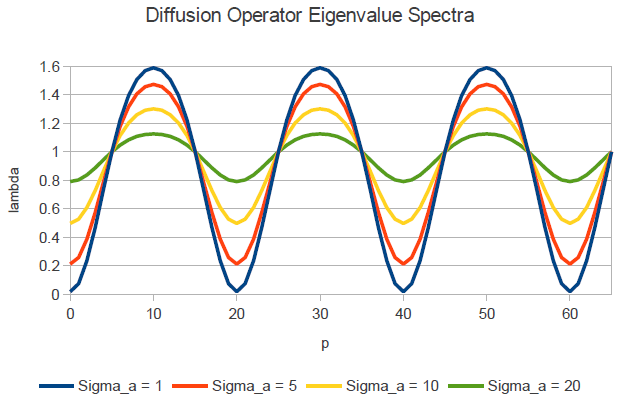
\includegraphics[width=5in,clip]{chapters/parallel_mc/diffusion_spectrum.png}
  \end{center}
  \caption{\textbf{Eigenvalue spectra for the diffusion equation.}}
  \label{fig:diffusion_spectrum}
\end{figure}
We find that the maximum eigenvalue exists when $p=q=0$, giving the
following for the spectral radius of the Jacobi preconditioned
iteration matrix:
\begin{equation}
  \rho(\ve{H}) = \frac{10 \alpha D}{3 h^2}\:.
  \label{eq:iteration_radius}
\end{equation}

\subsection{Neumann Series Convergence}
\label{subsec:neumann_convergence}
As outlined in \S\ref{sec:mc_preliminaries}, the adjoint Monte Carlo
method is effectively an approximation to a stationary method. In the
adjoint Neumann-Ulam method, $k$ iterations, equivalent to $k$
applications of the iteration matrix, are approximated by a random
walk of average length $k$ to yield the summation in
Eq~(\ref{eq:adjoint_neumann_solution})
\citep{dimov_new_1998,danilov_asymptotic_2000}. This random walk
length, or the number of transitions before the termination of a
history (either by the weight cutoff, absorption, or exiting the
global domain) is therefore approximately the number of stationary
iterations required to converge to the specified tolerance. In the
case of the adjoint Neumann-Ulam method, no such tolerance exists,
however, we have specified a weight cutoff, $W_c$, that determines
when low-weight histories will be prematurely terminated as their
contributions are deemed minute. After $k$ iterations, a stationary
method is terminated as the error has reached some fraction,
$\epsilon$, of the initial error:
\begin{equation}
  ||\ve{e}^{k}||_2 = \epsilon ||\ve{e}^0||_2\:.
  \label{eq:linear_k_iter_norm4}
\end{equation}
Per Eq~(\ref{eq:linear_k_iter_norm3}), we see that this fraction is
equivalent to $\epsilon = \rho(\ve{H})^k$. For the adjoint
Neumann-Ulam method, if we take this fraction to be the weight cutoff,
a measure of how accurately the contributions of a particular history
to the solution are tallied, we then have the following relationship
for $k$:
\begin{equation}
  k = \frac{ \log(W_c) }{ \log( \rho(\ve{H}) ) }\:.
  \label{eq:analytic_k}
\end{equation}
This then gives us a means to estimate the length of the random walks
that will be generated from a particular linear operator based on the
eigenvalues of its iteration matrix (independent of the linear
operator splitting chosen) and based on the weight cutoff parameter
used in the Neumann-Ulam method.

\subsection{Domain Leakage Approximations}
\label{subsec:domain_leak_approx}
In a domain decomposed situation, not all histories will remain within
the domain they started in and must instead be communicated. This
communication, expected to be expensive, was analyzed by Siegel and
colleagues for idealized, load balanced situations for full nuclear
reactor core Monte Carlo neutral particle simulations
\citep{siegel_analysis_2012}.  To quantify the number of particles
that leak out of the local domain they define a leakage fraction,
$\Lambda$, as:
\begin{equation}
  \Lambda = \frac{average\ \#\ of\ particles\ leaving\ local\ domain}
          {total\ of\ \#\ of\ particles\ starting\ in\ local\ domain}\:.
          \label{eq:leakage_fraction}
\end{equation}
For their studies, Siegel and colleagues assumed that the value of
$\Lambda$ was dependent on the total cross subsection of the system via
the Wigner rational approximation. Outlined more thoroughly by Hwang's
chapter in \citep{azmy_nuclear_2010}, we will use both the Wigner
rational approximation and the mean chord approximation as a means to
estimate the leakage fraction.

In the case of domain decomposed linear operator equations, we can use
diffusion theory to estimate the optical thickness of a domain in the
decomposition and the corresponding leakage fraction in terms of
properties of the linear operator and the discretization. To begin we
must first calculate the mean distance a Monte Carlo history will move
in the grid by computing the mean squared distance of its movement
along the chord of length $l$ defined across the domain. After a
single transition a history will have moved a mean squared distance
of:
\begin{equation}
  \langle \bar{r_1^2} \rangle = (n_s h)^2\:,
  \label{eq:step_1_length}
\end{equation}
where $h$ is the size of the discrete grid elements along the chord
and $n_s$ is the number of grid elements a history will move on
average every transition. For our diffusion model problem, $n_s$ would
equate to the expected number of states in the $i$ (or $j$ as the problem is
symmetric) direction that a history will move in a single
transition and is dependent on the stencil used for the
discretization. After $k$ transitions in the random walk, the history
will have moved a mean squared distance of:
\begin{equation}
  \langle \bar{r_k^2} \rangle = k (n_s h)^2\:.
  \label{eq:step_k_length}
\end{equation}
If our chord is of length $l$ and there are $n_i$ grid elements (or
states to which a history may transition) along that chord, then $h =
l / n_i$ giving:
\begin{equation}
  \langle \bar{r_k^2} \rangle = k \Bigg(\frac{n_s l}{n_i}\Bigg)^2\:.
  \label{eq:step_k_length_sub}
\end{equation}
From diffusion theory, we expect the average number of interactions
along the chord to be:
\begin{equation}
  \tau = \frac{l}{2 d \sqrt{\langle \bar{r_k^2} \rangle}}\:,
  \label{eq:optical_thickness_1}
\end{equation}
where $d$ is the dimensionality of the problem and $\sqrt{\langle
  \bar{r_k^2} \rangle}$ is effectively the mean free path of the Monte
Carlo history in the domain. We can readily interpret $\tau$ to be the
\textit{effective optical thickness} of a domain of length
$l$. Inserting Eq~(\ref{eq:step_k_length_sub}) we arrive at:
\begin{equation}
  \tau = \frac{n_i}{2 d n_s \sqrt{k}}\:,
  \label{eq:optical_thickness_2}
\end{equation}
which if expanded with Eq~(\ref{eq:analytic_k}) gives us the final
relation for the effective optical thickness:
\begin{equation}
  \tau = \frac{n_i}{2 d n_s}
  \sqrt{\frac{\log(\rho(\ve{H}))}{\log(W_c)}}\:.
  \label{eq:optical_thickness_3}
\end{equation}

For optically thin domains, we expect that most histories will be
communicated, while optically thick domains will leak the fraction of
histories that did not interact within. Using the optical thickness
defined in Eq~(\ref{eq:optical_thickness_3}), we can then complete the
leakage approximations by defining the bounds of $\tau \rightarrow 0,
\Lambda \rightarrow 1$ and $\tau \rightarrow \infty, \Lambda
\rightarrow \tau^{-1}$.  With these bounds we can then define the
leakage fraction out of a domain for the adjoint Neumann-Ulam method
using the Wigner rational approximation:
\begin{equation}
  \Lambda = \frac{1}{1+\tau}\:,
  \label{eq:wigner_domain_leakage}
\end{equation}
and using the mean-chord approximation:
\begin{equation}
  \Lambda = \frac{1-e^{-\tau}}{\tau}\:.
  \label{eq:mean_chord_domain_leakage}
\end{equation}
Here, the leakage fraction is explicitly bound to the eigenvalues of
the iteration matrix, the size of the domain, the content of the
discretization stencil, and the weight cutoff selected to terminate
low weight histories.

\subsection{Numerical Experiments}
\label{subsec:numerical_experiments}
To test the relationships developed by the spectral analysis, we form
two simple numerical experiments using the diffusion model problem:
one to measure the length of the random walks as a function of the
iteration matrix eigenvalues, and one to measure the domain leakage
fraction as a function of the iteration matrix eigenvalues and the
discretization properties. Before doing this, we verify our
computation of the spectral radius of the iteration matrix by
numerically computing the largest eigenvalue of the diffusion operator
using an iterative eigenvalue solver. For this verification, a $100
\times 100$ square grid with $h=0.01$, $h=0.1$, and $h=1.0$ and the
absorption cross varied from 0 to 100 while the scattering cross
subsection was fixed at unity. Figure~\ref{fig:measured_spec_rad} gives
the measured spectral radius of the iteration matrix and the computed
spectral radius for the preconditioned diffusion operator using
Eq~(\ref{eq:iteration_radius}) as function of the absorption to
scattering ratio $(\Sigma_a / \Sigma_s)$. Excellent agreement was
observed between the analytic and numerical results with all data
points computed within the tolerance of the iterative eigenvalue
solver.
\begin{figure}[t!]
  \begin{spacing}{1.0}
    \begin{center}
      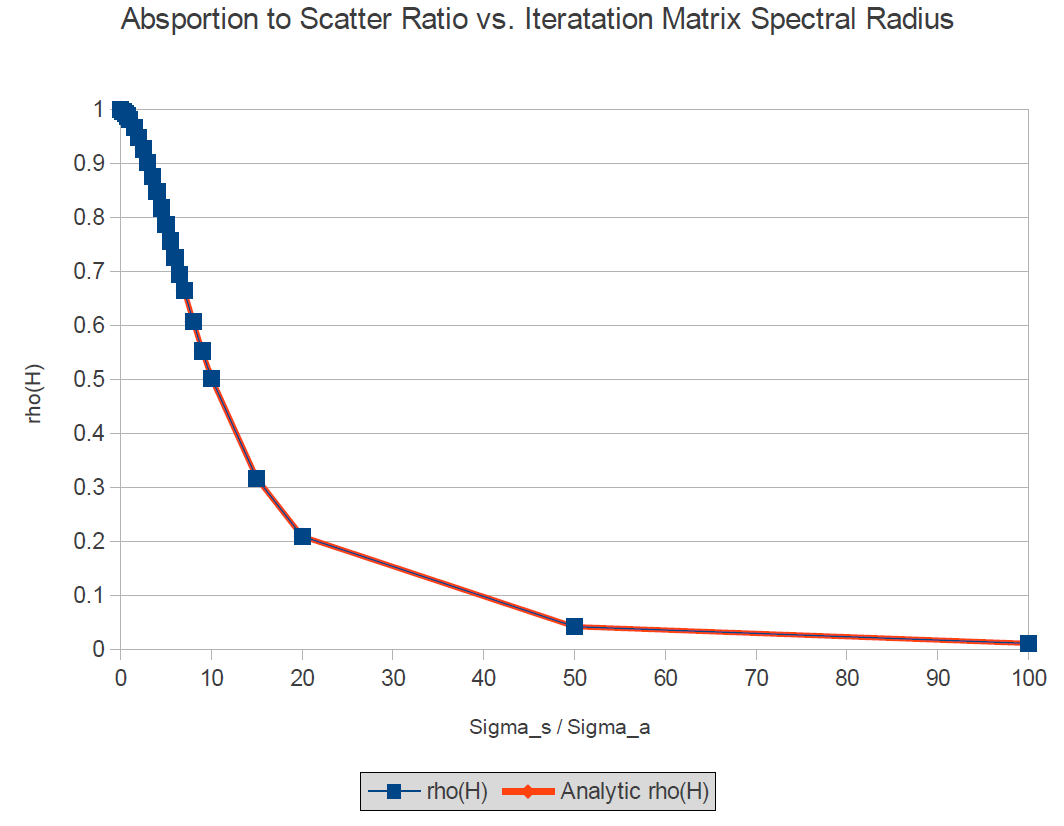
\includegraphics[width=5in,clip]{chapters/parallel_mc/measured_spec_rad.png}
    \end{center}
    \caption{\textbf{Measured and analytic preconditioned diffusion
        operator spectral radius as a function of the absorption cross
        subsection to scattering cross subsection ratio.} \textit{Values of
        $h=0.01$, $h=0.1$, and $h=1.0$ were used. The red data was
        computed numerically by an eigensolver while the black dashed
        data was generated by Eq~(\ref{eq:iteration_radius}).}}
    \label{fig:measured_spec_rad}
  \end{spacing}
\end{figure}

\subsubsection{Random Walk Length}
\label{subsubsec:walk_length}
With the eigenvalue derivations verified, we can go about setting up
an experiment to measure the length of the random walks generated by
the adjoint Neumann-Ulam solver. To do this, we again use a $100
\times 100$ square grid with $h=0.1$ and the absorption cross varied
from 0 to 100 while the scattering cross subsection was fixed at
unity. Three weight cutoff values of \sn{1}{-2}, \sn{1}{-4}, and
\sn{1}{-8} were used with 10,000 histories generated by a point source
of strength 1 in the center of the domain. For each of the histories,
the number of transitions made was tallied to provide an effective
value of $k$ for each history. This value was then averaged over all
histories to get a measured value of $k$ for the particular
operator. On the left, Figure~\ref{fig:measured_length} presents these
measurements as well as the analytic result computed by
Eq~(\ref{eq:analytic_k}) as a function of the iteration matrix
spectral radius, $\rho(\ve{H})$. On the right,
Figure~\ref{fig:measured_length} gives the relative difference between the
predicted and observed results. We note good qualitative agreement
between the measured and analytic results. However, we observe a
larger relative difference for both long and short random walks.
\begin{figure}[t!]
  \begin{spacing}{1.0}
    \begin{center}
      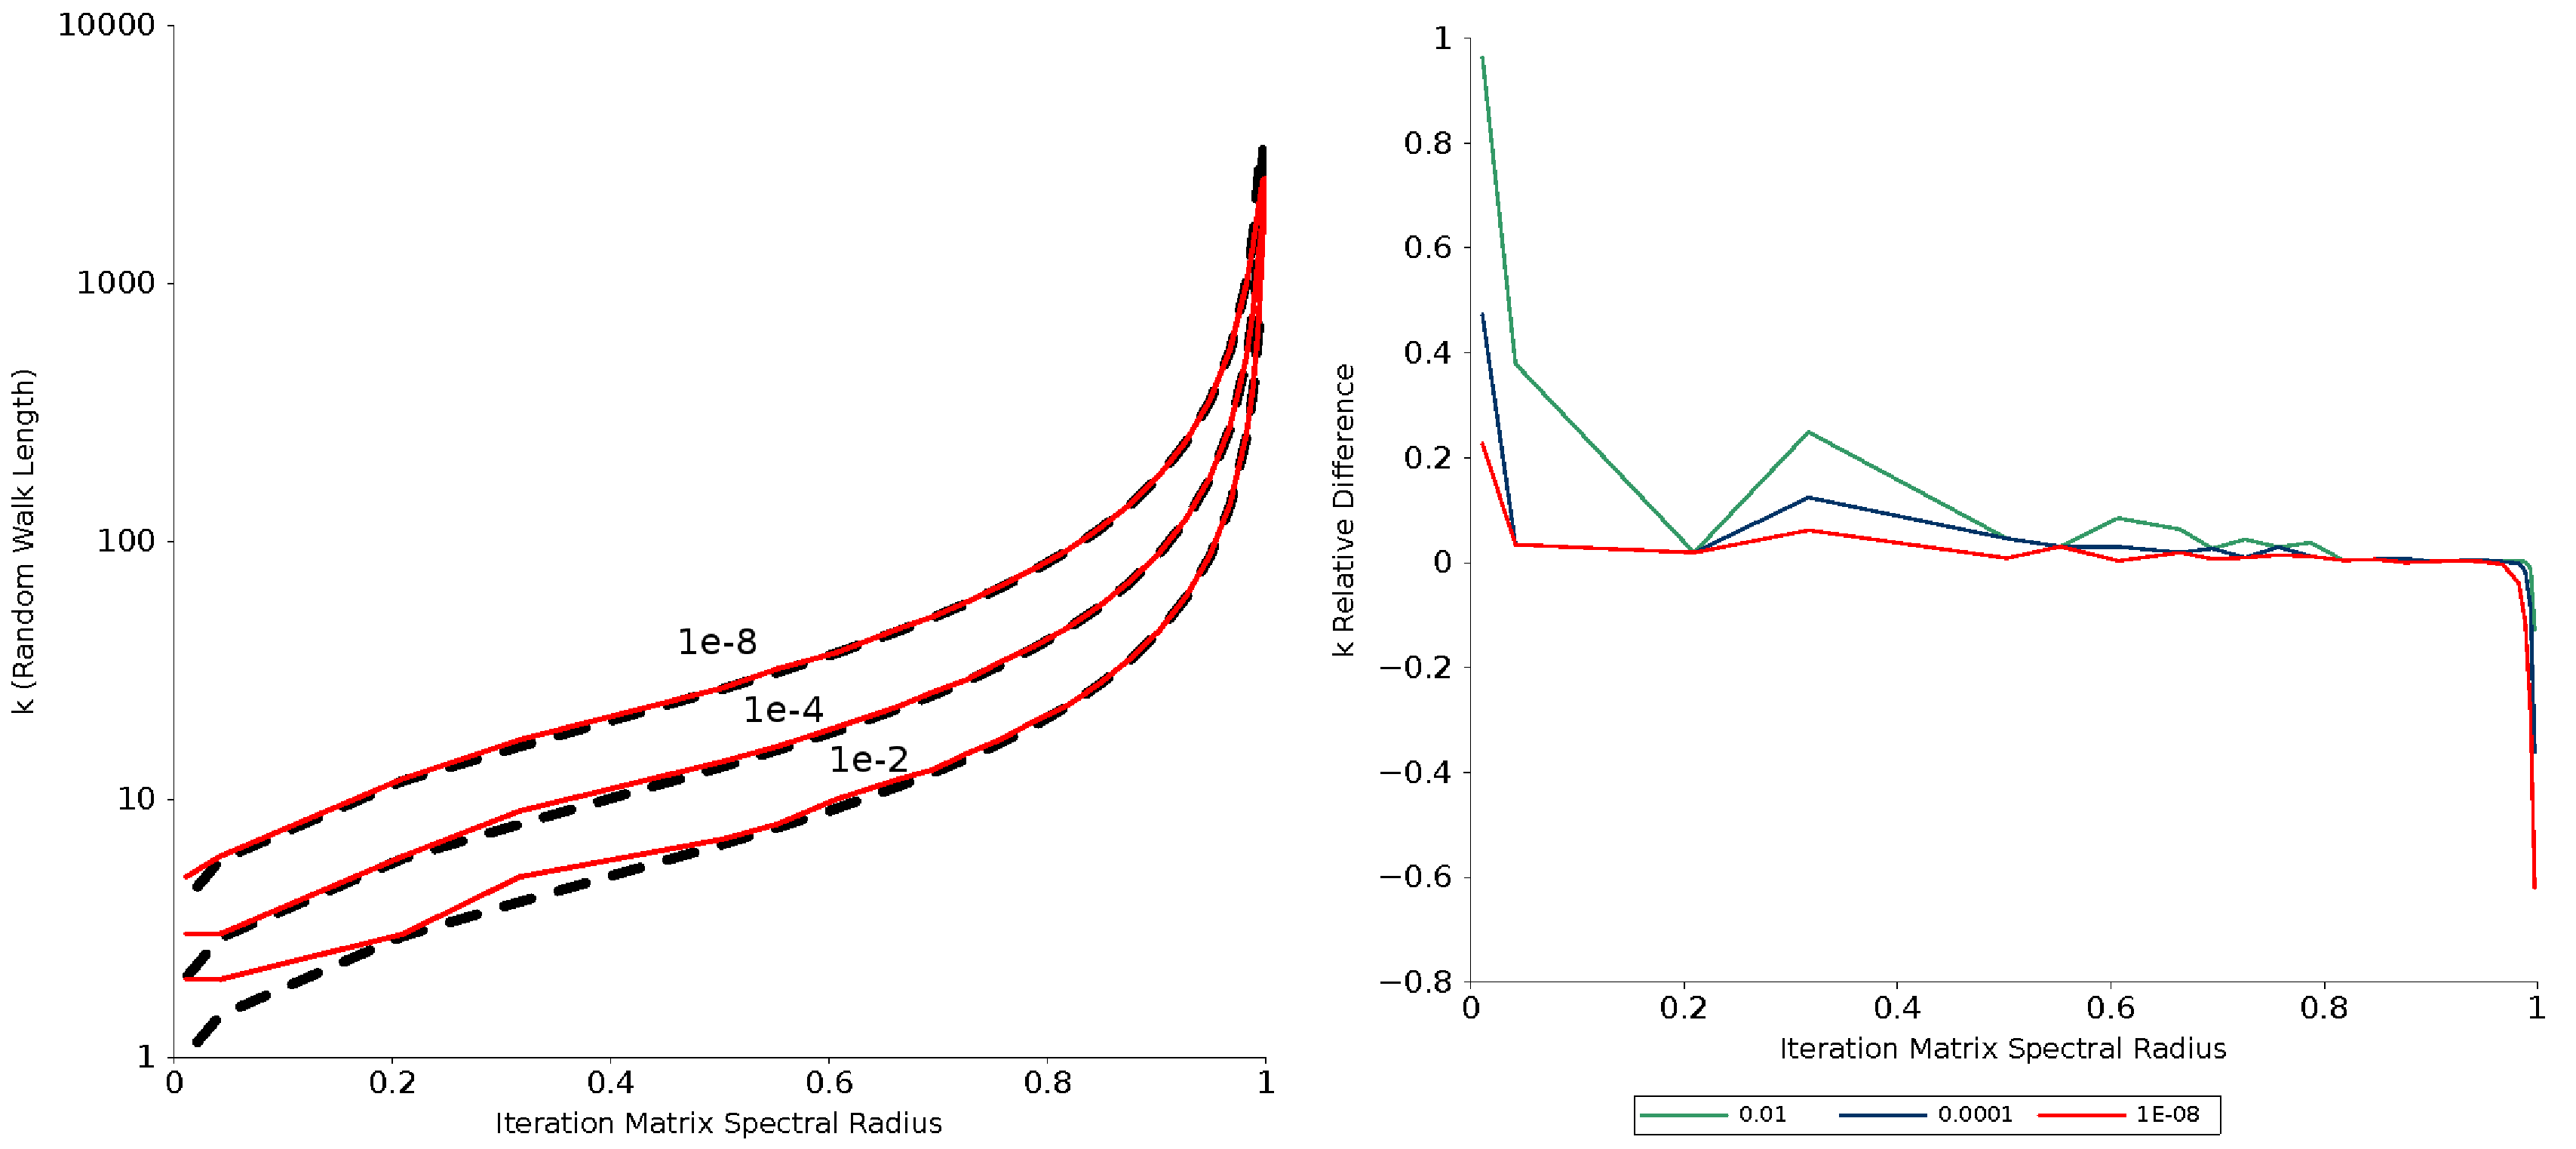
\includegraphics[width=6.0in,clip]{chapters/parallel_mc/measured_length_2.pdf}
    \end{center}
    \caption{\textbf{Measured and analytic random walk length as a
        function of the iteration matrix spectral radius.} \textit{The
        weight cutoff was varied with \sn{1}{-2}, \sn{1}{-4}, and
        \sn{1}{-8}. In the left plot, the red data was computed
        numerically by an adjoint Neumann-Ulam implementation while
        the black dashed data was generated by
        Eq~(\ref{eq:analytic_k}). In the right plot, the relative
        difference between the predicted and measured results is
        presented for each weight cutoff.}}
    \label{fig:measured_length}
  \end{spacing}
\end{figure}

\subsubsection{Domain Leakage}
\label{subsubsec:domain_leakage}
Finally, we seek to measure the leakage from a domain in a domain
decomposed Monte Carlo calculation and assess the quality of our
analytic relation for the optical thickness of a domain and the
associated leakage approximations. For this experiment, a square grid
with $h=0.1$ was decomposed into 9 square domains, 3 in each cardinal
direction with measurements occurring in the central domain without
boundary grid points. For the cross subsections, the absorption cross
subsection was varied from 1 to 100 while the scattering cross
subsection was set to zero to create a purely absorbing environment
with weight cutoff of \sn{1}{-4}. The optical thickness of these
domains will vary as a function of the absorption cross subsection if
the other parameters are fixed. To compute the optical thickness,
along with the spectral radius as given by
Eq~(\ref{eq:iteration_radius}), we also need the parameters $n_i$ and
$n_s$ which respectively describe the typical domain length and the
average number of states moved along that typical length per history
transition. For our grid above, the domains are varied in size with
$50 \times 50$, $100 \times 100$, and $200 \times 200$ cells giving
$n_i=50$, $n_i=100$, and $n_i=200$ grid points or states along the
typical length of the domain respectively. Looking at the Laplacian
stencil in Eq~(\ref{eq:nine_point_stencil}), we see that all history
transitions will only move a single state in either the $i$ or $j$
directions due to the symmetry of the problem. Furthermore, if we
choose the $i$ direction, not all states we will transition to will
move the history in that direction. Therefore, we look to the
definition of the iteration matrix in Eq~(\ref{eq:iteration_stencil})
and the definition of the adjoint probability matrix in
Eq~(\ref{eq:adjoint_probability}) to estimate the $n_s$ parameter. For
a particular transition starting at state $(i,j)$, 6 of the 8 possible
new states in the stencil move the history in $i$ direction with
relative coefficients of 4 for moving in the $(\pm i,0)$ direction and
of 1 for moving in the $(\pm i,\pm j)$. These coefficients dictate the
frequency those states are visited relative to the others. For those 6
states we can visit along the typical length, their sum is 12 out of
the total 20 for the coefficients for all possible states with their
ratio giving $n_s = \frac{3}{5}$.

To compute the leakage fraction numerically, \sn{3}{5} histories were
sampled from a uniform source of strength unity over the global
domain. At the start of a stage of histories, the number of histories
starting in the center domain was computed and as the stage
progressed, the number of histories that exited that domain was
tallied with the ratio of the two numbers providing a numerical
measure for the leakage fraction. Figure~\ref{fig:measured_leakage}
gives the domain leakage measurements for the domain in the center of
the global grid as well as the analytic result computed by
Eqs~(\ref{eq:wigner_domain_leakage}) and
(\ref{eq:mean_chord_domain_leakage}) as a function of the iteration
matrix spectral radius.
\begin{figure}[t!]
  \begin{spacing}{1.0}
    \begin{center}
      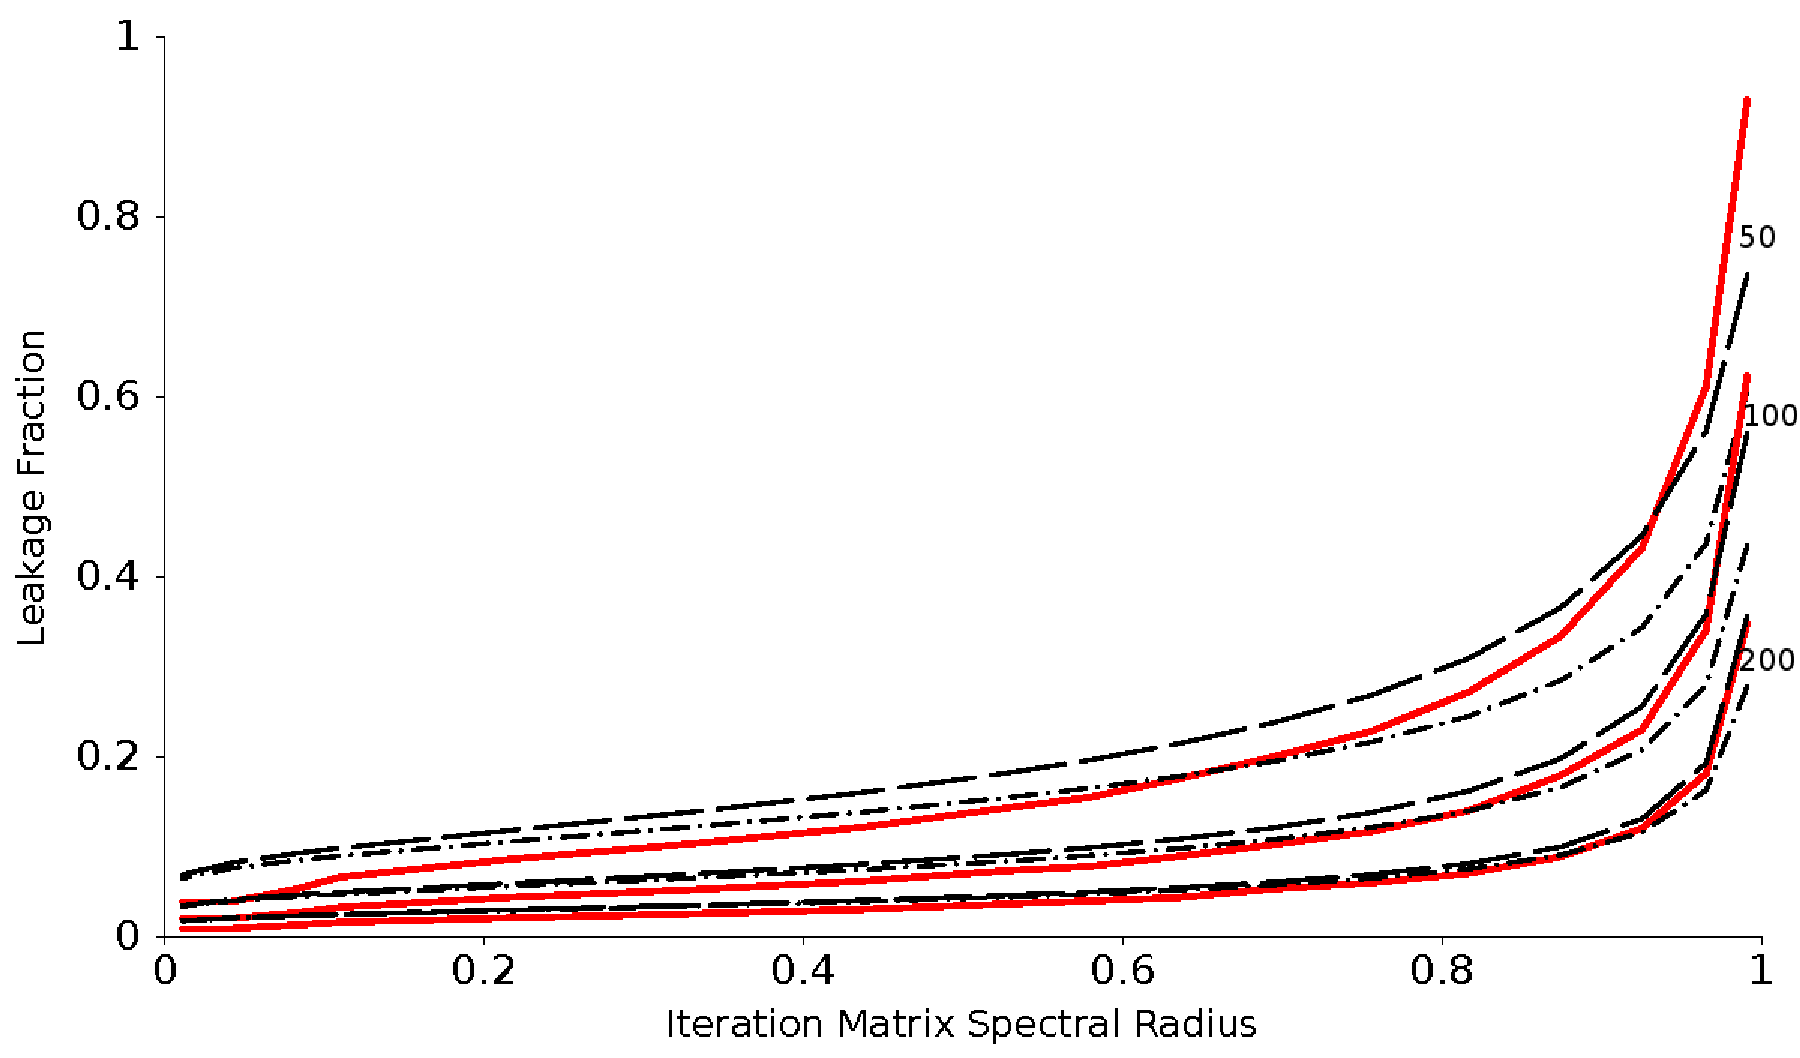
\includegraphics[width=6.0in,clip]{chapters/parallel_mc/leakage_variation_2.pdf}
    \end{center}
    \caption{\textbf{Measured and analytic domain leakage as a
        function of the iteration matrix spectral radius.} \textit{To
        test the behavior with respect to domain size, $n_i=50$,
        $n_i=100$,and $n_i=200$ were used. The red data was computed
        numerically by a domain-decomposed adjoint Neumann-Ulam
        implementation, the black dashed data was generated by
        Eq~(\ref{eq:mean_chord_domain_leakage}) using the mean-chord
        approximation, and the dashed-dotted black data was generated
        by Eq~(\ref{eq:wigner_domain_leakage}) using the Wigner
        rational approximation.}}
    \label{fig:measured_leakage}
  \end{spacing}
\end{figure}
Again, we note good qualitative agreement between the measured and
analytic quantities but we begin to see the limits of the leakage
approximations. To compare the quality of the two approximations, the
absolute difference between the computed leakage fraction and that
generated by the Wigner rational and mean chord approximations is
plotted in Figure~\ref{fig:leakage_error} for all domain sizes
tested. 
\begin{figure}[t!]
  \begin{spacing}{1.0}
    \begin{center}
      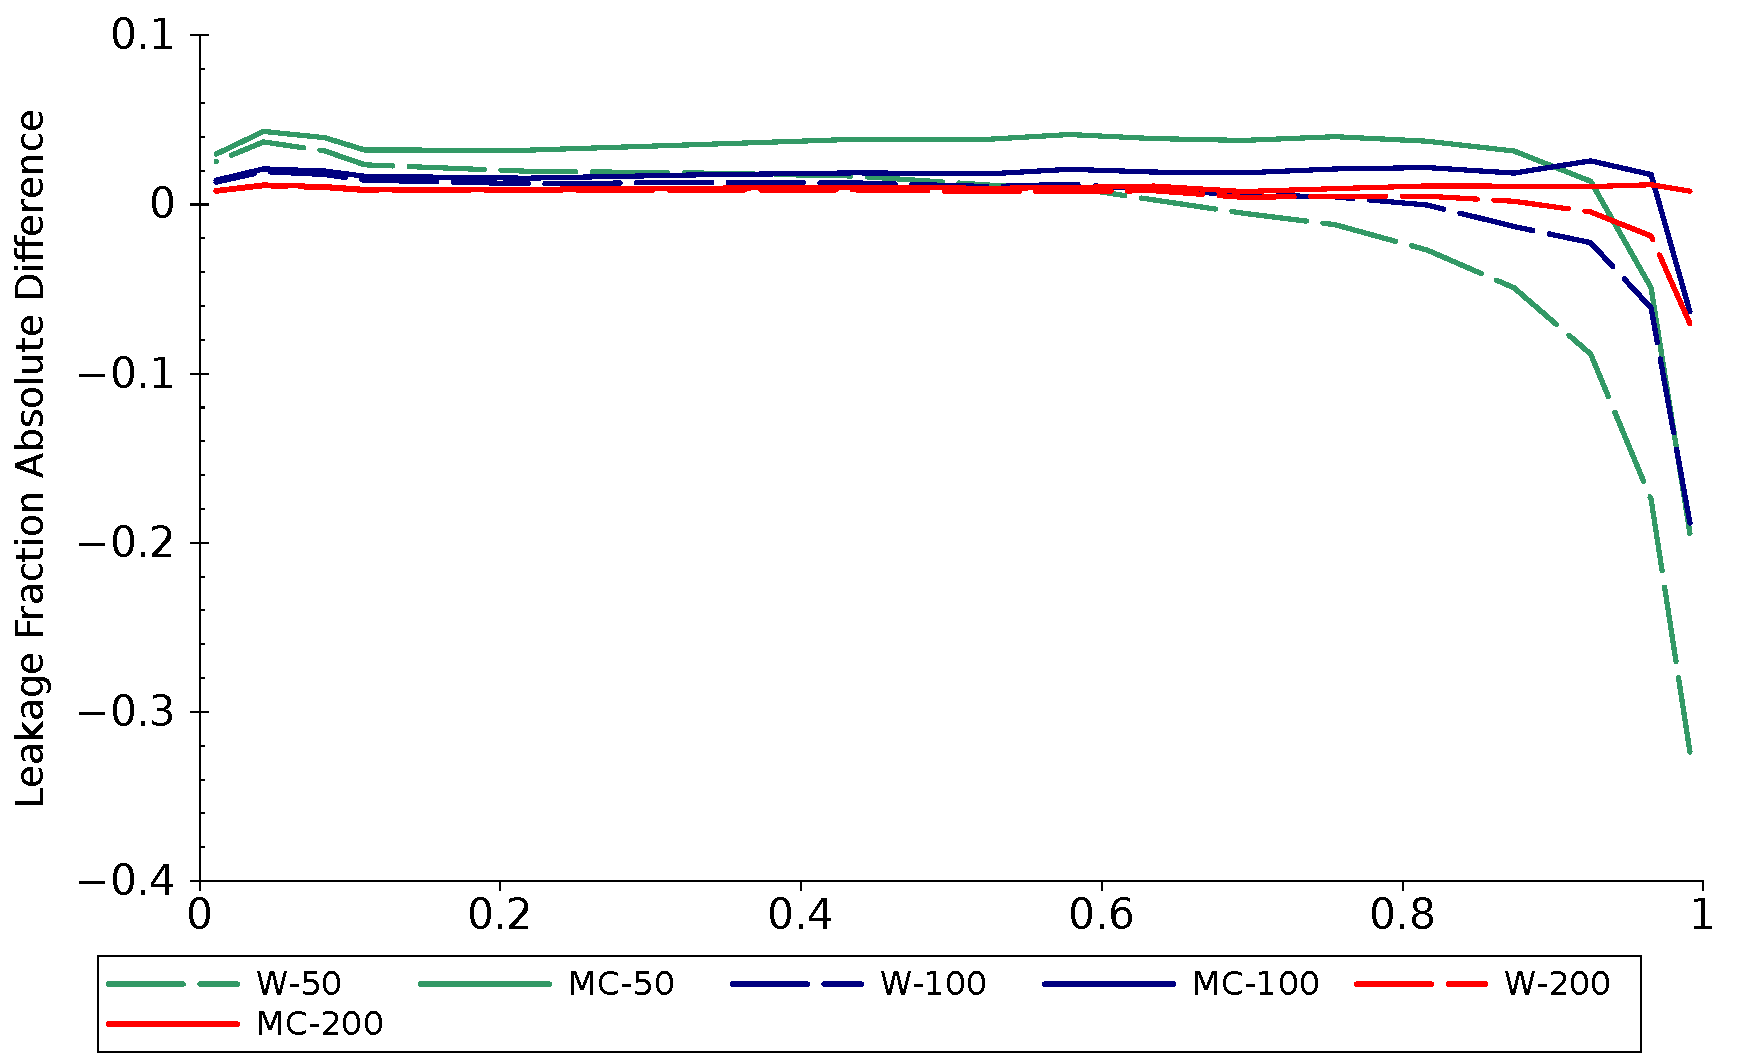
\includegraphics[width=6.0in,clip]{chapters/parallel_mc/leakage_error_2.pdf}
    \end{center}
    \caption{\textbf{Measured and analytic domain leakage absolute
        difference as a function of the iteration matrix spectral radius.}
      \textit{To test the behavior with respect to domain size,
        $n_i=50$ (green), $n_i=100$ (blue), and $n_i=200$ (red) were
        used. The dashed lines represent the difference using the Wigner
        rational approximation while the solid lines represent the
        difference using the mean-chord approximation.}}
    \label{fig:leakage_error}
  \end{spacing}
\end{figure}
From these difference results, the mean chord approximation is shown to
have a lower difference for ill-conditioned systems as compared to the
Wigner approximation while the Wigner approximation produces less
difference for more well-conditioned systems. We also note that for the
optically thick domains, the difference is likely corresponded to that
observed in Figure~\ref{fig:measured_length} for the $k$ parameter
while the large relative difference in $k$ for optically thin domains does
not affect the approximation significantly. In general, the mean chord
approximation is a better choice to estimate the leakage fraction in a
domain from the adjoint Neumann-Ulam method and except for a single
data point with $n_i=50$, the mean chord approximation yielded leakage
fractions within 0.05 of the measured results. As the domain becomes
more optically thick (with both increasing $n_i$ and decreasing
$\rho(\ve{H})$), the approximations are more accurate.

%%---------------------------------------------------------------------------%%
\section{Fully Asynchronous Neumann-Ulam Algorithm}
\label{sec:asynchronous_algorithm}

In the context of radiation transport, in 2009 Brunner and colleagues
provided a fully asynchronous domain decomposed parallel aglorithm as
implemented in production implicit Monte Carlo codes
\citep{brunner_efficient_2009}. In their work they identify two data
sets that are required to be communicated: the sharing of particles
that are transported from one domain to another and therefore from one
processor to another and a global communication that signals if
particle transport has been completed on all processors. Although the
implementation was robust and allowed for scaling to large numbers of
processors, performance issues were still noted with parallel
efficiency improvements needed in both the weak and strong scaling
cases for unbalanced problems. These results led Brunner to conclude
that a combination of domain decomposition and domain replication
could be used to solve some of these issues.

We can take much of what was learned from Brunner's parallel Monte
Carlo method for radiation transport and directly apply it to a
parallel formulation of the Neumann-Ulam method. Direct analogs can be
derived from these works by noting that the primary difference between
solving a linear system with Monte Carlo methods and fixed source
Monte Carlo transport problems is the content of the Markov chains
that are generated. The transitions represented by these chains are
bound by probabilities and weights and are initiated by the sampling
of a source. In the context of transport problems, those transitions
represent events such as particle scattering and absorption with
probabilities that are determined by physical data in the form of
cross sections. For stochastic matrix inversion, those transitions
represent moving between the equations of the linear system (and
therefore the physical domain which they represent) and their
probabilities are defined by the coefficients of those
equations. Ultimately, we tally the contributions to generate
expectation values in the desired states as we progress through the
chains. Therefore, parallel methods for Monte Carlo radiation
transport can be abstracted and we can use those concepts that apply
to matrix inversion methods as an initial means of developing a
parallel Neumann-Ulam-type solver. In this section the fully
asynchronous MSOD Neumann-Ulam algorithm developed for this work is
presented step-by-step in detail.

\subsection{Generating the Transport Domain with Preconditioning}
\label{subsec:domain_generation}

\subsection{Generating the Transport Source with Preconditioning}
\label{subsec:source_generation}

\subsection{Transition Processing Kernel}
\label{subsec:transition_processing}
Processing the transition of a single stochastic history from one
state to another in the system is the fundamental kernel of the
transport procedure. In this kernel, an incoming history has a state
consisting of the current discrete state in the system in which it
resides and its current weight and is processed as given by
Algorithm~\ref{alg:transition_process}.
\begin{algorithm}[h!]
  \caption{Stochastic History Transition Processing Kernel}
  \label{alg:power_iteration}
  \begin{algorithmic}
    \State processTransition( history ):
    \State i = history.state
    \State j = sampleRowCDF( C[i] )
    \State history.state = j
    \State history.weight *= w[i,j]
  \end{algorithmic}
  \label{alg:transition_process}
\end{algorithm}
The core component here is the sampling of the CDF for a particular
state generated by the probablities from the Neumann-Ulam
decomposition. Upon exiting, the kernel has modified the state of the
history with a new state and multiplied the weight with the
corresponding transition weight to form the product in
Eq~(\ref{eq:direct_permutation_weight}).

\subsection{Local Domain Transport Kernel}
\label{subsec:local_domain_transport}

\subsection{Domain-to-Domain Communication Kernel}
\label{subsec:domain_to_domain_kernel}

\subsection{Asynchronous Transport Kernel}
\label{subsec:async_transport_kernel}

%%---------------------------------------------------------------------------%%
\subsection{Multiple-Set Overlapping-Domain Neumann-Ulam Algorithm}
\label{subsec:msod}
In 2010, Wagner and colleagues developed the \textit{multiple-set
  overlapping-domain} (MSOD) decomposition for parallel Monte Carlo
applications for full-core light water reactor analysis
\citep{wagner_hybrid_2010}. In their work, an extension of Brunner's,
their scheme employed similar parallel algorithms for particle
transport but a certain amount of overlap between adjacent domains was
used to decrease the number of particles leaving the local domain. In
addition, Wagner utilized a level of replication of the domain such
that the domain was only decomposed on $O(100)$ processors and if
replicated $O(1,000)$ times achieves simulation on $O(100,000)$
processors, thus providing spatial and particle parallelism. Each
collection of processors that constitutes a representation of the
entire domain is referred to as a set, and within a set overlap occurs
among its sub-domains. The original motivation was to decompose the
domain in a way that it remained in a physical cabinet in a large
distributed machine, thus reducing latency costs during
communication. A multiple set scheme is also motivated by the fact
that communication during particle transport only occurs within a set,
limiting communications during the transport procedure to a group of
$O(100)$ processors, a number that was shown to have excellent
parallel efficiencies in Brunner's work and therefore will scale well
in this algorithm. The overlapping domains within each set also
demonstrated reduced communication costs. On each processor, the
source is sampled in the local domain that would exist if no overlap
was used while tallies can be made over the entire overlapping domain.

To demonstrate this, consider the example adapted from Mervin's work
with Wagner and others in the same area \citep{mervin_variance_2012}
and presented in Figure~\ref{fig:msod_example}.
\begin{figure}[t!]
  \begin{center}
    \scalebox{1.5}{
      \input{chapters/parallel_mc/msod_example.pdftex_t} }
  \end{center}
  \caption{\textbf{Overlapping domain example illustrating how domain
      overlap can reduce communication costs.}
    \textit{All particles start in the blue region of interest. The
      dashed line represents 0.5 domain overlap between domains.}}
  \label{fig:msod_example}
\end{figure}
In this example, 3 particle histories are presented emanating from the
blue region of interest. Starting with particle A, if no domain
overlap is used then the only the blue domain exists on the starting
processor. Particle A is then transported through 3 other domains
before the history ends, therefore requiring three communications to
occur in Brunner's algorithm. If a 0.5 domain overlap is permitted as
shown by the dashed line, then the starting process owns enough of the
domain such that no communications must occur in order to complete the
particle A transport process. Using 0.5 domain overlap also easily
eliminates cases such as the represented by the path of particle C. In
this case, particle C is scattering between two adjacent domains,
incurring a large latency cost for a single particle. Finally, with
particle B we observe that 0.5 domain overlap will still not eliminate
all communications. However, if 1 domain overlap were used, the entire
geometry shown in Figure~\ref{fig:msod_example} would be contained on
the source processor and therefore transport of all 3 particles
without communication would occur.

Wagner and colleagues used this methodology for a 2-dimensional
calculation of a pressurized water reactor core and varied the domain
overlap from 0 to 3 domain overlap (a $7 \times 7$ box in the context
of our example) where a domain constituted a fuel assembly. For the
fully domain decomposed case, they observed that 76.12\% of all source
particles leave the domain. At 1.5 domain overlap, the percentage of
source particles born in the center assembly leaving the processor
domain dropped to 1.05\% and even further for 0.02\% for the 3 domain
overlap. Based on these results, this overlap approach, coupled with
the multiple sets paradigm that will scale for existing parallel
transport algorithms, provides a scalable Monte Carlo algorithm for
today's modern machines.

\subsection{Generating Overlap}
\label{subsec:msod_overlap}

\subsection{Generating Multiple Sets}
\label{subsec:msod_sets}

\subsection{MSOD Neumann Ulam Algorithm}
\label{subsec:msod_algorithm}

%%---------------------------------------------------------------------------%%
\section{Parallel MCSA}
\label{sec:parallel_mcsa}
With the parallel adjoint Neumann-Ulam solver implementation described
aboive, the parallel implementation of the MCSA method is
trivial. Recall the MCSA iteration procedure outlined in
Eq~(\ref{eq:mcsa}). In \S\ref{sec:parallel_krylov_methods} we
discussed parallel matrix and vector operations as utilized in
conventional Krylov methods. We utilize these here for the parallel
MCSA implementation. In the first step, a parallel matrix-vector
multiply is used to apply the split operator to the previous iterate's
solution. A parallel vector update is then performed with the source
vector to arrive at the initial iteration guess. In the next step, the
residual is computed by the same operations where now the operator is
applied to the solution guess with a parallel matrix-vector multiply
and then a parallel vector update with the source vector is
performed. Once the correction is computed with a parallel adjoint
Neumann-Ulam solve, this correction is applied to the guess with a
parallel vector update to get the new iteration
solution. Additionally, as given by
Eq~(\ref{eq:mcsa_stopping_criteria}), 2 parallel vector reductions
will be required to check the stopping criteria: one initially to
compute the infinity norm of the source vector, and another at every
iteration to compute the infinity norm of the residual vector. For
this implementation, all of the issues that will be potentially
generated by the parallel adjoint solver implementation will manifest
themselves here as the quality of the correction will be of intense
study.

%%---------------------------------------------------------------------------%%
\section{Parallel MCSA Verification}
\label{sec:parallel_verification}

%%---------------------------------------------------------------------------%%
\section{Small Cluster Scaling Studies}
\label{sec:small_scaling_studies}

%%---------------------------------------------------------------------------%%
\section{Leadership-Class Parallel Scaling Studies}
\label{sec:leadership_scaling_studies}
For all cases, we explore scaling for just the Monte Carlo transport
kernel and MCSA as a whole iterative scheme. This will be necessary to
determine if the initial relaxation step required at each iteration is
a limiting factor in convergence. For each case, it will be
constructive to study the scaling performance as a function of
spectral radius - dictated by the cross sections and grid size to
diffusion length ratio. In addition, all of these studies should
hopefully have data from both the cluster and Titan and should all be
compared to Aztec GMRES and CG implementations with appropriate
preconditioning.

\subsection{Titan}
\label{subsec:titan}

\subsection{Communication Parameters}
\label{subsec:comm_parameters}

\subsection{Pure Domain Decomposition}
\label{subsec:pure_domain_decomp}

\subsubsection{Weak Scaling}
\label{subsubsec:pure_weak}

\subsubsection{Strong Scaling}
\label{subsubsec:pure_strong}

\subsection{Overlapping Domain Decomposition}
\label{subsec:overlapping_domain_decomp}

\subsubsection{Weak Scaling}
\label{subsubsec:overlapping_weak}

\subsubsection{Strong Scaling}
\label{subsubsec:overlapping_strong}

\subsection{MSOD Decomposition}
\label{subsec:msod_decomposition}

\subsubsection{Weak Scaling}
\label{subsubsec:msod_weak}

\subsubsection{Strong Scaling}
\label{subsubsec:msod_strong}

%%---------------------------------------------------------------------------%%
\section{Multiple Fuel Assembly $SP_N$ Challenge Problem}
\label{sec:spn_challenge_problem}
